% Created by tikzDevice version 0.12
% !TEX encoding = UTF-8 Unicode
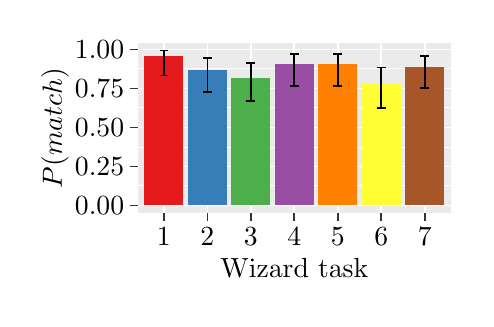
\begin{tikzpicture}[x=1pt,y=1pt]
\definecolor{fillColor}{RGB}{255,255,255}
\path[use as bounding box,fill=fillColor,fill opacity=0.00] (0,0) rectangle (158.40, 97.89);
\begin{scope}
\path[clip] (  0.00,  0.00) rectangle (158.40, 97.89);
\definecolor{drawColor}{RGB}{255,255,255}
\definecolor{fillColor}{RGB}{255,255,255}

\path[draw=drawColor,line width= 0.6pt,line join=round,line cap=round,fill=fillColor] (  0.00,  0.00) rectangle (158.40, 97.89);
\end{scope}
\begin{scope}
\path[clip] ( 39.80, 30.86) rectangle (152.90, 92.39);
\definecolor{fillColor}{gray}{0.92}

\path[fill=fillColor] ( 39.80, 30.86) rectangle (152.90, 92.39);
\definecolor{drawColor}{RGB}{255,255,255}

\path[draw=drawColor,line width= 0.3pt,line join=round] ( 39.80, 40.71) --
	(152.90, 40.71);

\path[draw=drawColor,line width= 0.3pt,line join=round] ( 39.80, 54.80) --
	(152.90, 54.80);

\path[draw=drawColor,line width= 0.3pt,line join=round] ( 39.80, 68.90) --
	(152.90, 68.90);

\path[draw=drawColor,line width= 0.3pt,line join=round] ( 39.80, 82.99) --
	(152.90, 82.99);

\path[draw=drawColor,line width= 0.6pt,line join=round] ( 39.80, 33.66) --
	(152.90, 33.66);

\path[draw=drawColor,line width= 0.6pt,line join=round] ( 39.80, 47.75) --
	(152.90, 47.75);

\path[draw=drawColor,line width= 0.6pt,line join=round] ( 39.80, 61.85) --
	(152.90, 61.85);

\path[draw=drawColor,line width= 0.6pt,line join=round] ( 39.80, 75.95) --
	(152.90, 75.95);

\path[draw=drawColor,line width= 0.6pt,line join=round] ( 39.80, 90.04) --
	(152.90, 90.04);

\path[draw=drawColor,line width= 0.6pt,line join=round] ( 49.23, 30.86) --
	( 49.23, 92.39);

\path[draw=drawColor,line width= 0.6pt,line join=round] ( 64.94, 30.86) --
	( 64.94, 92.39);

\path[draw=drawColor,line width= 0.6pt,line join=round] ( 80.64, 30.86) --
	( 80.64, 92.39);

\path[draw=drawColor,line width= 0.6pt,line join=round] ( 96.35, 30.86) --
	( 96.35, 92.39);

\path[draw=drawColor,line width= 0.6pt,line join=round] (112.06, 30.86) --
	(112.06, 92.39);

\path[draw=drawColor,line width= 0.6pt,line join=round] (127.77, 30.86) --
	(127.77, 92.39);

\path[draw=drawColor,line width= 0.6pt,line join=round] (143.48, 30.86) --
	(143.48, 92.39);
\definecolor{fillColor}{RGB}{228,26,28}

\path[fill=fillColor] ( 42.16, 33.66) rectangle ( 56.30, 87.48);
\definecolor{fillColor}{RGB}{55,126,184}

\path[fill=fillColor] ( 57.87, 33.66) rectangle ( 72.01, 82.52);
\definecolor{fillColor}{RGB}{77,175,74}

\path[fill=fillColor] ( 73.58, 33.66) rectangle ( 87.71, 79.79);
\definecolor{fillColor}{RGB}{152,78,163}

\path[fill=fillColor] ( 89.28, 33.66) rectangle (103.42, 84.67);
\definecolor{fillColor}{RGB}{255,127,0}

\path[fill=fillColor] (104.99, 33.66) rectangle (119.13, 84.67);
\definecolor{fillColor}{RGB}{255,255,51}

\path[fill=fillColor] (120.70, 33.66) rectangle (134.84, 77.51);
\definecolor{fillColor}{RGB}{166,86,40}

\path[fill=fillColor] (136.41, 33.66) rectangle (150.54, 83.78);
\definecolor{drawColor}{RGB}{0,0,0}

\path[draw=drawColor,line width= 0.6pt,line join=round] ( 47.66, 89.59) --
	( 50.80, 89.59);

\path[draw=drawColor,line width= 0.6pt,line join=round] ( 49.23, 89.59) --
	( 49.23, 80.62);

\path[draw=drawColor,line width= 0.6pt,line join=round] ( 47.66, 80.62) --
	( 50.80, 80.62);

\path[draw=drawColor,line width= 0.6pt,line join=round] ( 63.37, 86.92) --
	( 66.51, 86.92);

\path[draw=drawColor,line width= 0.6pt,line join=round] ( 64.94, 86.92) --
	( 64.94, 74.54);

\path[draw=drawColor,line width= 0.6pt,line join=round] ( 63.37, 74.54) --
	( 66.51, 74.54);

\path[draw=drawColor,line width= 0.6pt,line join=round] ( 79.07, 85.13) --
	( 82.22, 85.13);

\path[draw=drawColor,line width= 0.6pt,line join=round] ( 80.64, 85.13) --
	( 80.64, 71.30);

\path[draw=drawColor,line width= 0.6pt,line join=round] ( 79.07, 71.30) --
	( 82.22, 71.30);

\path[draw=drawColor,line width= 0.6pt,line join=round] ( 94.78, 88.30) --
	( 97.92, 88.30);

\path[draw=drawColor,line width= 0.6pt,line join=round] ( 96.35, 88.30) --
	( 96.35, 76.77);

\path[draw=drawColor,line width= 0.6pt,line join=round] ( 94.78, 76.77) --
	( 97.92, 76.77);

\path[draw=drawColor,line width= 0.6pt,line join=round] (110.49, 88.30) --
	(113.63, 88.30);

\path[draw=drawColor,line width= 0.6pt,line join=round] (112.06, 88.30) --
	(112.06, 76.77);

\path[draw=drawColor,line width= 0.6pt,line join=round] (110.49, 76.77) --
	(113.63, 76.77);

\path[draw=drawColor,line width= 0.6pt,line join=round] (126.20, 83.44) --
	(129.34, 83.44);

\path[draw=drawColor,line width= 0.6pt,line join=round] (127.77, 83.44) --
	(127.77, 68.91);

\path[draw=drawColor,line width= 0.6pt,line join=round] (126.20, 68.91) --
	(129.34, 68.91);

\path[draw=drawColor,line width= 0.6pt,line join=round] (141.90, 87.69) --
	(145.05, 87.69);

\path[draw=drawColor,line width= 0.6pt,line join=round] (143.48, 87.69) --
	(143.48, 76.03);

\path[draw=drawColor,line width= 0.6pt,line join=round] (141.90, 76.03) --
	(145.05, 76.03);
\end{scope}
\begin{scope}
\path[clip] (  0.00,  0.00) rectangle (158.40, 97.89);
\definecolor{drawColor}{RGB}{0,0,0}

\node[text=drawColor,anchor=base east,inner sep=0pt, outer sep=0pt, scale=  1.00] at ( 34.85, 30.22) {0.00};

\node[text=drawColor,anchor=base east,inner sep=0pt, outer sep=0pt, scale=  1.00] at ( 34.85, 44.31) {0.25};

\node[text=drawColor,anchor=base east,inner sep=0pt, outer sep=0pt, scale=  1.00] at ( 34.85, 58.41) {0.50};

\node[text=drawColor,anchor=base east,inner sep=0pt, outer sep=0pt, scale=  1.00] at ( 34.85, 72.50) {0.75};

\node[text=drawColor,anchor=base east,inner sep=0pt, outer sep=0pt, scale=  1.00] at ( 34.85, 86.60) {1.00};
\end{scope}
\begin{scope}
\path[clip] (  0.00,  0.00) rectangle (158.40, 97.89);
\definecolor{drawColor}{gray}{0.20}

\path[draw=drawColor,line width= 0.6pt,line join=round] ( 37.05, 33.66) --
	( 39.80, 33.66);

\path[draw=drawColor,line width= 0.6pt,line join=round] ( 37.05, 47.75) --
	( 39.80, 47.75);

\path[draw=drawColor,line width= 0.6pt,line join=round] ( 37.05, 61.85) --
	( 39.80, 61.85);

\path[draw=drawColor,line width= 0.6pt,line join=round] ( 37.05, 75.95) --
	( 39.80, 75.95);

\path[draw=drawColor,line width= 0.6pt,line join=round] ( 37.05, 90.04) --
	( 39.80, 90.04);
\end{scope}
\begin{scope}
\path[clip] (  0.00,  0.00) rectangle (158.40, 97.89);
\definecolor{drawColor}{gray}{0.20}

\path[draw=drawColor,line width= 0.6pt,line join=round] ( 49.23, 28.11) --
	( 49.23, 30.86);

\path[draw=drawColor,line width= 0.6pt,line join=round] ( 64.94, 28.11) --
	( 64.94, 30.86);

\path[draw=drawColor,line width= 0.6pt,line join=round] ( 80.64, 28.11) --
	( 80.64, 30.86);

\path[draw=drawColor,line width= 0.6pt,line join=round] ( 96.35, 28.11) --
	( 96.35, 30.86);

\path[draw=drawColor,line width= 0.6pt,line join=round] (112.06, 28.11) --
	(112.06, 30.86);

\path[draw=drawColor,line width= 0.6pt,line join=round] (127.77, 28.11) --
	(127.77, 30.86);

\path[draw=drawColor,line width= 0.6pt,line join=round] (143.48, 28.11) --
	(143.48, 30.86);
\end{scope}
\begin{scope}
\path[clip] (  0.00,  0.00) rectangle (158.40, 97.89);
\definecolor{drawColor}{RGB}{0,0,0}

\node[text=drawColor,anchor=base,inner sep=0pt, outer sep=0pt, scale=  1.00] at ( 49.23, 19.03) {1};

\node[text=drawColor,anchor=base,inner sep=0pt, outer sep=0pt, scale=  1.00] at ( 64.94, 19.03) {2};

\node[text=drawColor,anchor=base,inner sep=0pt, outer sep=0pt, scale=  1.00] at ( 80.64, 19.03) {3};

\node[text=drawColor,anchor=base,inner sep=0pt, outer sep=0pt, scale=  1.00] at ( 96.35, 19.03) {4};

\node[text=drawColor,anchor=base,inner sep=0pt, outer sep=0pt, scale=  1.00] at (112.06, 19.03) {5};

\node[text=drawColor,anchor=base,inner sep=0pt, outer sep=0pt, scale=  1.00] at (127.77, 19.03) {6};

\node[text=drawColor,anchor=base,inner sep=0pt, outer sep=0pt, scale=  1.00] at (143.48, 19.03) {7};
\end{scope}
\begin{scope}
\path[clip] (  0.00,  0.00) rectangle (158.40, 97.89);
\definecolor{drawColor}{RGB}{0,0,0}

\node[text=drawColor,anchor=base,inner sep=0pt, outer sep=0pt, scale=  1.00] at ( 96.35,  7.44) {Wizard task};
\end{scope}
\begin{scope}
\path[clip] (  0.00,  0.00) rectangle (158.40, 97.89);
\definecolor{drawColor}{RGB}{0,0,0}

\node[text=drawColor,rotate= 90.00,anchor=base,inner sep=0pt, outer sep=0pt, scale=  1.00] at ( 12.39, 61.63) {\(P(match)\)};
\end{scope}
\end{tikzpicture}
